\section{Flujo de trabajo en GIT}
\frame
{
\frametitle{Flujo de trabajo en GIT}
\begin{center}
 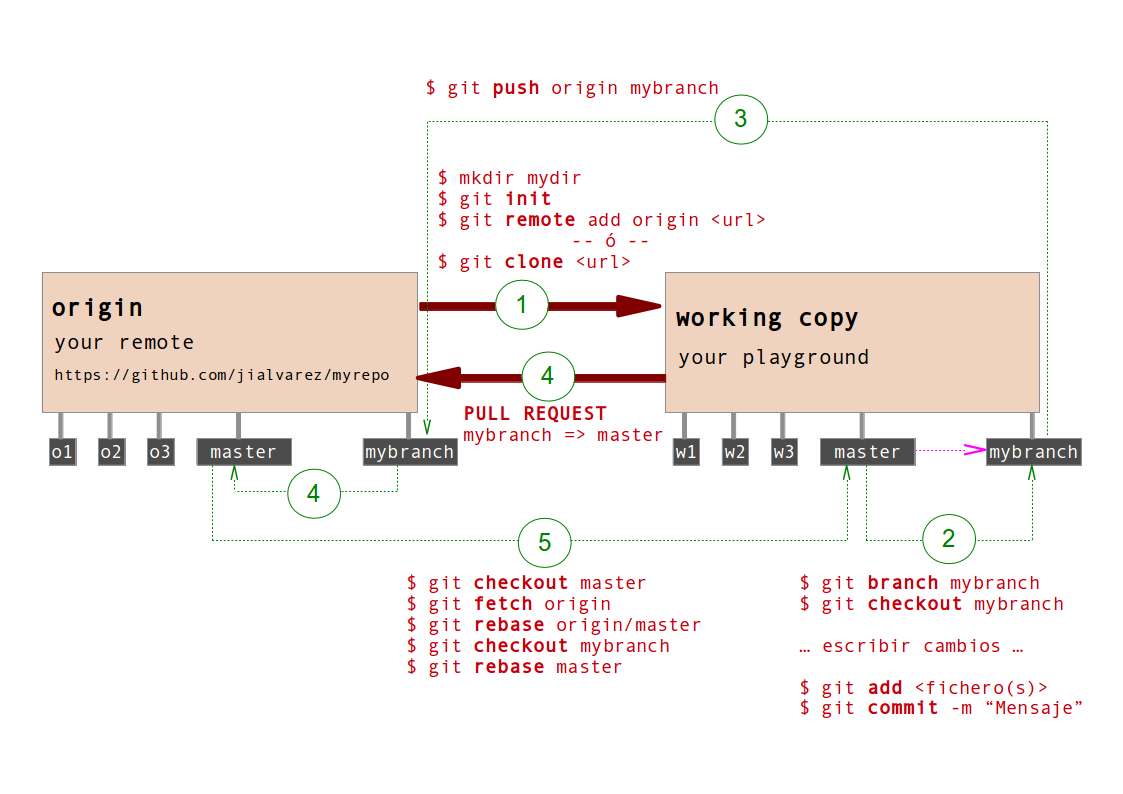
\includegraphics[height=7cm]{imgs/gitworkflow.png}
\end{center}
}

\frame
{
\frametitle{Git branching}

\begin{tabular}[t]{m{5cm}m{6cm}}
   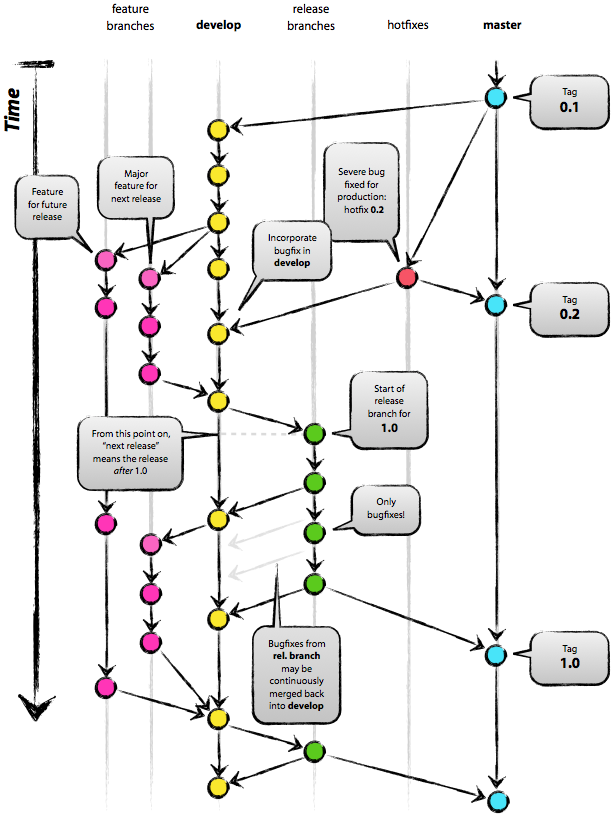
\includegraphics[height=8cm]{imgs/gitbranching.png} 
   &
   \begin{itemize}
    \addtolength{\itemindent}{0.4cm}
    \item Reglas base comunes propuestas por Vincent Driessen en 2010 para organizar el trabajo en equipo
    \item Ramas master (commits producción) y develop (siguiente versión planificada)
    \item Ramas master (commits producción) y develop (siguiente versión planificada)
   \end{itemize}
\end{tabular}
}

\frame
{
\frametitle{Etapas de un fichero (I)}
\# \textbf{Archivos sin seguimiento:}\\
\#   (use git add <archivo>... para incluir lo que se ha de ejecutar)\\
\#\\
\#	\textcolor{red}{fichero.tex}\\
}

\frame
{
\frametitle{Etapas de un fichero (II)}
\# \textbf{Cambios no preparados para el commit:}\\
\#   (use git add <archivo>... para actualizar lo que se ejecutará)\\
\#   (use git checkout $--$ <archivo>... para descartar cambios en el directorio de trabajo)\\
\#\\
\#	\textcolor{red}{modificado:   advanced.tex}\\
\#	\textcolor{red}{modificado:   principal.pdf}\\
\#\\
}

\frame
{
\frametitle{Etapas de un fichero (III)}
\# \textbf{Cambios para hacer commit:}\\
\#   (use git reset HEAD <archivo>...para eliminar stage)\\
\#\\
\#	\textcolor{green}{modificado:   workflow.tex}\\
\#\\
}
